\documentclass[11pt,a4paper]{article}
\usepackage[T1]{fontenc}
\usepackage{tgpagella}
\usepackage{mathpazo}
\usepackage[margin=23mm,headheight=16pt]{geometry}
\usepackage{microtype,amsmath,amssymb,mathtools,booktabs,longtable,array,multicol}
\usepackage{xcolor,tikz,pgfplots,fancyhdr,titlesec,enumitem,hyperref}
\usetikzlibrary{arrows.meta,positioning,calc,decorations.pathreplacing}
\pgfplotsset{compat=1.18}
\definecolor{deep}{HTML}{173C68}\definecolor{violet}{HTML}{7151AA}\definecolor{muted}{HTML}{556574}
\hypersetup{colorlinks=true,linkcolor=deep,urlcolor=violet}
\titleformat{\section}{\Large\bfseries\color{deep}}{\thesection.}{.6em}{}
\titleformat{\subsection}{\large\bfseries\color{deep}}{\thesubsection}{.6em}{}
\setlength{\parindent}{0pt}\setlength{\parskip}{5pt}
\setlist[itemize]{itemsep=2pt,topsep=2pt}
\pagestyle{fancy}\fancyhf{}\fancyhead[L]{\small Quantum Physics Companion}\fancyhead[R]{\small Optical Lattices IV}\fancyfoot[C]{\thepage}
\newcounter{example}\newenvironment{worked}[1]{\refstepcounter{example}\par\medskip\noindent\textbf{\color{violet}Worked Example \theexample. #1}\par\smallskip}{\par\medskip}
\newcommand{\op}[1]{\hat{#1}}
\usepackage{amsthm}
\newtheorem{supplexample}{Supplementary Worked Example}
\begin{document}
\begin{center}
{\Large\color{deep}\bfseries THE QUANTUM PHYSICS COMPANION}\par\vspace{5mm}
{\huge\bfseries Quantum Phase Transitions\\[2mm] and Excitations in Optical Lattices}\par\vspace{4mm}
{\large Chapter IV: An Exact Route from Two Rubidium Atoms to Many-Body Dynamics}\par\vspace{4mm}
{\color{muted}Rb-87 $\cdot$ Bose--Hubbard theory $\cdot$ exact diagonalization $\cdot$ quasiparticles $\cdot$ quantum quenches}\par\vspace{3mm}
\rule{.76\linewidth}{.6pt}
\end{center}
\begin{abstract}
This chapter starts from two bosons on two sites and derives the exact spectrum, eigenstates, double occupancy, number fluctuations and coherence. It then develops finite three-site diagonalization, strong-coupling excitations, lattice Bogoliubov modes, the thermodynamic superfluid--Mott transition, quantum quenches, and collapse--revival dynamics. All ``orbitals'' in the Bose--Hubbard description refer to the center-of-mass motion of complete neutral atoms, not to electronic $5s$ or $5p$ orbitals inside rubidium. Formulae and finite-size limits are stated explicitly, with worked examples and references.
\end{abstract}
\tableofcontents\newpage
\section{Physical setting and the Bose--Hubbard Hamiltonian}
A deep far-detuned optical lattice supplies a periodic potential for the motion of neutral $^{87}$Rb atoms. In the lowest-band Wannier basis, retaining onsite contact interactions and nearest-neighbor hopping, a uniform system is modeled by
\begin{equation}\boxed{\hat H=-J\sum_{\langle i,j\rangle}(\hat a_i^\dagger\hat a_j+\hat a_j^\dagger\hat a_i)+\frac U2\sum_i\hat n_i(\hat n_i-1)-\mu\sum_i\hat n_i.}\end{equation}
The bond sum counts each undirected nearest-neighbor link once. The hopping scale $J>0$ favors delocalized atoms, while $U>0$ discourages multiple occupancy. The atomic field describes centers of mass: the internal electron configuration $[\mathrm{Kr}]5s^1$ remains associated with individual rubidium atoms.

\begin{center}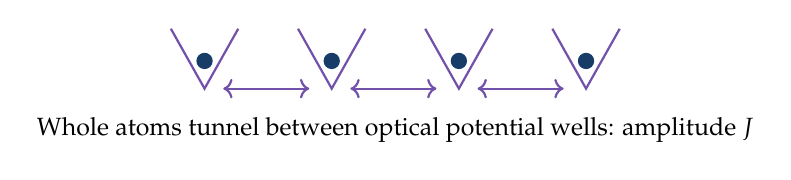
\begin{tikzpicture}[scale=.95]
\foreach \x in {0,1.7,3.4,5.1}{\draw[violet,thick] (\x,1)--(\x+.45,.2)--(\x+.9,1);}
\foreach \x in {.45,2.15,3.85,5.55}{\fill[deep] (\x,.57) circle (3.1pt);}
\foreach \a/\b in {.7/1.85,2.4/3.55,4.1/5.25}{\draw[<->,violet,thick] (\a,.2) -- (\b,.2);}
\node at (3,-.35){\small Whole atoms tunnel between optical potential wells: amplitude $J$};
\end{tikzpicture}\end{center}
\section{Exact diagonalization: two atoms on two sites}
Work at fixed $N=2$ and omit the constant chemical-potential contribution. A Fock basis is $\mathcal B=(|2,0\rangle,|1,1\rangle,|0,2\rangle)$. Since $\hat a|n\rangle=\sqrt n\,|n-1\rangle$ and $\hat a^\dagger|n\rangle=\sqrt{n+1}\,|n+1\rangle$, the exact matrix is
\begin{equation}\boxed{H=\begin{pmatrix}U&-\sqrt2J&0\\-\sqrt2J&0&-\sqrt2J\\0&-\sqrt2J&U\end{pmatrix}.}\end{equation}
For $|S\rangle=(|2,0\rangle+|0,2\rangle)/\sqrt2$ and $|A\rangle=(|2,0\rangle-|0,2\rangle)/\sqrt2$, the antisymmetric state has energy $E_A=U$, while $(|S\rangle,|1,1\rangle)$ carries the block $\left(\begin{smallmatrix}U&-2J\\-2J&0\end{smallmatrix}\right)$. Writing $D=\sqrt{U^2+16J^2}$, we obtain
\begin{equation}\boxed{E_\pm=\frac{U\pm D}{2},\qquad E_A=U.}\end{equation}
For $U\ge0$, $J>0$, the ground state $|G\rangle$ has $E_-$. In the phase convention of positive coefficients,
\begin{equation}
|G\rangle=\sqrt{1-P_{11}}\,|S\rangle+\sqrt{P_{11}}\,|1,1\rangle,\quad
\boxed{P_{11}=\frac12\left(1+\frac{U}{D}\right).}
\end{equation}
The probability of $|2,0\rangle$ or $|0,2\rangle$ individually is $(1-P_{11})/2$.
\begin{worked}{Noninteracting and strong-coupling limits}
For $U=0$, $D=4J$, $E_-=-2J$ and $|G\rangle=\tfrac12|2,0\rangle+\tfrac1{\sqrt2}|1,1\rangle+\tfrac12|0,2\rangle$. This is two bosons in the bonding orbital $(\phi_L+\phi_R)/\sqrt2$. For $U/J\to\infty$, $P_{11}\to1$ and $|G\rangle\to|1,1\rangle$. The finite dimer has a smooth crossover, not a thermodynamic phase transition.
\end{worked}
\begin{worked}{Numerical ground-state occupation}
Set $U=4J$. Then $D=4\sqrt2J$, $E_-/J=2-2\sqrt2\simeq-0.8284$, and $P_{11}=\tfrac12(1+1/\sqrt2)\simeq0.8536$.
\end{worked}
\begin{center}\begin{tabular}{rrrrr}\toprule
$U/J$ & $E_-/J$ & $P_{11}$ & $\langle K\rangle$ & $\langle D_n^2\rangle$\\\midrule
0&-2.0000&0.5000&2.0000&2.0000\\
1&-1.5616&0.6213&1.9403&1.5149\\
2&-1.2361&0.7236&1.7889&1.1056\\
4&-0.8284&0.8536&1.4142&0.5858\\
8&-0.4721&0.9472&0.8944&0.2111\\
20&-0.1980&0.9903&0.3922&0.0388\\\bottomrule
\end{tabular}\end{center}
\section{Exact coherence, correlations, and gaps}
Define $K=\hat a_1^\dagger\hat a_2+\hat a_2^\dagger\hat a_1$ and $D_n=\hat n_1-\hat n_2$. Hellmann--Feynman gives $\partial_JE_-=-\langle K\rangle$, and thus
\begin{equation}\boxed{\langle K\rangle=\frac{8J}{D},\qquad \langle D_n^2\rangle=2\left(1-\frac UD\right).}\end{equation}
By exchange symmetry $\langle n_1\rangle=\langle n_2\rangle=1$, and $\langle a_1^\dagger a_2\rangle=4J/D$. The $2\times2$ one-body density matrix has eigenvalues $1\pm4J/D$, which interpolate between $(2,0)$ at $U=0$ and $(1,1)$ as $U/J\to\infty$.
\begin{worked}{One-body natural-orbital occupations}
At $U=4J$, $D=4\sqrt2J$ and $\langle a_1^\dagger a_2\rangle=1/\sqrt2$. Natural occupations are $1\pm1/\sqrt2\simeq1.7071,0.2929$. These quantify the loss of single-mode condensation in the dimer, without implying its atoms change electronic $5s$ orbitals.
\end{worked}
\begin{worked}{Exact excitation gaps of the dimer}
The three levels are $E_-$, $U$, $E_+$. At $U\ge0$, $E_+\ge U$, so the first gap is $\Delta_1=U-E_-=(U+D)/2$; the gap to the upper symmetric eigenstate is $\Delta_2=E_+-E_-=D$. These are finite-size excitation gaps, not a bulk Mott gap.
\end{worked}
\begin{center}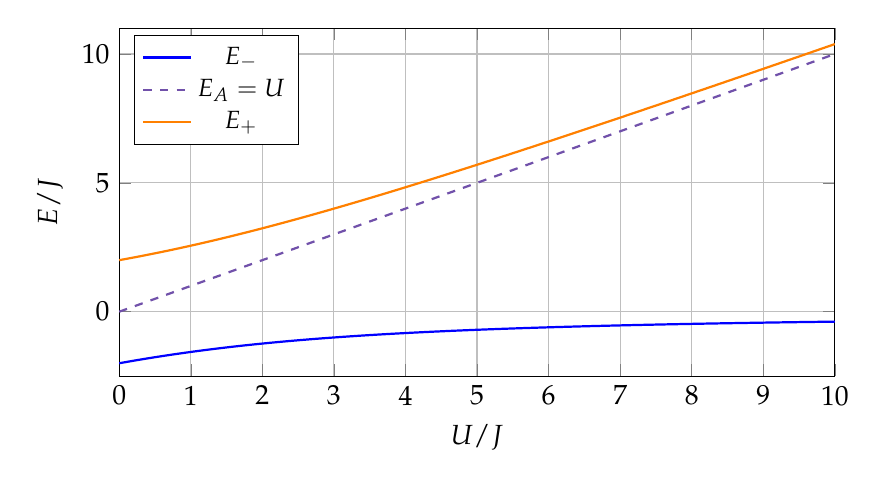
\begin{tikzpicture}\begin{axis}[width=.88\linewidth,height=6cm,xlabel={$U/J$},ylabel={$E/J$},xmin=0,xmax=10,ymin=-2.5,ymax=11,grid=major,legend style={font=\small,at={(.02,.98)},anchor=north west}]
\addplot[blue,thick,domain=0:10,samples=100]{(x-sqrt(x*x+16))/2};\addlegendentry{$E_-$}
\addplot[violet,dashed,thick,domain=0:10]{x};\addlegendentry{$E_A=U$}
\addplot[orange,thick,domain=0:10,samples=100]{(x+sqrt(x*x+16))/2};\addlegendentry{$E_+$}
\end{axis}\end{tikzpicture}\end{center}
\section{Three sites and general finite-size diagonalization}
For $L$ lattice sites with $N$ identical bosons, fixed-$N$ Fock states $|n_1,\dots,n_L\rangle$ obey $\sum_i n_i=N$, yielding
\begin{equation}\boxed{\dim\mathcal H_{N,L}=\binom{N+L-1}{L-1}.}\end{equation}
For $N=2,L=3$ there are six states: $|200\rangle,|020\rangle,|002\rangle,|110\rangle,|101\rangle,|011\rangle$. With open boundaries, hopping occurs only across the bonds $1$--$2$ and $2$--$3$. A matrix element taking $|\ldots,n_i,n_j,\ldots\rangle$ to $|\ldots,n_i+1,n_j-1,\ldots\rangle$ equals $-J\sqrt{(n_i+1)n_j}$.
\begin{worked}{Six-dimensional Hamiltonian for two bosons on three sites}
Take the ordered basis $(|200\rangle,|020\rangle,|002\rangle,|110\rangle,|101\rangle,|011\rangle)$. The matrix is
\[\small H=\begin{pmatrix}
U&0&0&-\sqrt2J&0&0\\
0&U&0&-\sqrt2J&0&-\sqrt2J\\
0&0&U&0&0&-\sqrt2J\\
-\sqrt2J&-\sqrt2J&0&0&-J&0\\
0&0&0&-J&0&-J\\
0&-\sqrt2J&-\sqrt2J&0&-J&0
\end{pmatrix}.\]
Every entry follows from bosonic square-root occupation factors. At $U=0$, the single-particle open-chain energies are $-\sqrt2J,0,+\sqrt2J$, so both bosons in the lowest orbital have ground energy $-2\sqrt2J$.
\end{worked}
\begin{worked}{Hilbert-space size and computational scaling}
For $N=3,L=3$, $\dim\mathcal H=\binom52=10$; for $N=10,L=10$, $\dim\mathcal H=\binom{19}{9}=92378$. Fixed-number exact diagonalization grows rapidly, motivating sparse matrices, symmetries, tensor networks, and quantum Monte Carlo.
\end{worked}
\section{Strong-coupling Mott excitations}
At zero hopping $J=0$, the energy of one site with $n$ bosons in the grand canonical description is $E_n=U n(n-1)/2-\mu n$. An integer-filling Mott region $n_0$ is locally stable when
\begin{equation}U(n_0-1)<\mu<U n_0.\end{equation}
The local particle and hole costs are
\begin{equation}\boxed{\Delta_p^{(0)}=Un_0-\mu,\qquad\Delta_h^{(0)}=\mu-U(n_0-1).}\end{equation}
At $J=0$, a spatially separated particle--hole pair costs $U$ irrespective of $\mu$. For weak nonzero hopping, particle and hole excitations disperse; to first order on a hypercubic lattice in $d$ dimensions,
\begin{align}
\epsilon_p(\mathbf k)&\simeq Un_0-\mu-2J(n_0+1)\sum_{\alpha=1}^d\cos(k_\alpha a),\\
\epsilon_h(\mathbf k)&\simeq\mu-U(n_0-1)-2Jn_0\sum_{\alpha=1}^d\cos(k_\alpha a).
\end{align}
These are lowest-order strong-coupling approximations, not exact expressions near the critical point.
\begin{worked}{One particle--hole excitation at unit filling}
At $n_0=1$ and $J=0$, $|\dots1,1,\dots\rangle\to|\dots0,2,\dots\rangle$ costs $U$. Setting $\mu=U/2$, particle and hole additions each cost $U/2$; their sum is $U$.
\end{worked}
\section{Weakly interacting superfluid: lattice Bogoliubov modes}
In a homogeneous superfluid at mean occupancy $n$, the nearest-neighbor tight-binding dispersion measured relative to its minimum is
\begin{equation}\epsilon_{\mathbf k}=2J\sum_{\alpha=1}^d[1-\cos(k_\alpha a)].\end{equation}
The Bogoliubov spectrum, for a stable weakly interacting condensate, is
\begin{equation}\boxed{E_B(\mathbf k)=\sqrt{\epsilon_{\mathbf k}(\epsilon_{\mathbf k}+2Un)}.}\end{equation}
For $|k_\alpha a|\ll1$, $\epsilon_{\mathbf k}\simeq Ja^2|\mathbf k|^2$ and $E_B\simeq\hbar c|\mathbf k|$ with
\begin{equation}\boxed{c=\frac a\hbar\sqrt{2JUn}.}\end{equation}
This gapless phonon is a collective density/phase excitation. It is distinct from the gapped single-site particle--hole excitations deep in a Mott insulator.
\begin{worked}{Sound velocity estimate}
Take $a=532$ nm, $J/h=100$ Hz, $U/h=1000$ Hz, $n=1$. Then $c=(a/\hbar)\sqrt{2JUn}\simeq1.26$ mm/s. This is a parameter illustration, not a specified experimental calibration. The Bogoliubov approximation requires conditions compatible with a coherent weakly depleted phase.
\end{worked}
\section{Thermodynamic quantum phase transition}
A two-site or three-site finite system crosses over smoothly; the sharp superfluid--Mott transition appears in the thermodynamic limit at commensurate filling. In mean-field decoupling, $\hat a_i^\dagger\hat a_j\approx\psi(\hat a_i^\dagger+\hat a_j)-\psi^2$ for real uniform order parameter $\psi=\langle\hat a_i\rangle$. Expanding the single-site energy near $\psi=0$ gives a transition criterion at the tip of the $n$th Mott lobe:
\begin{equation}\boxed{\left(\frac{U}{zJ}\right)^{\rm MF}_{c}=(\sqrt{n+1}+\sqrt n)^2,}\end{equation}
where $z$ is the number of nearest neighbors. For $n=1$, the mean-field value is $U/(zJ)=3+2\sqrt2\simeq5.828$. On a three-dimensional simple cubic lattice ($z=6$), it predicts $U/J\simeq34.97$. Quantum Monte Carlo instead gives $(U/J)_c=29.34(2)$ at the unit-filling lobe tip (Capogrosso-Sansone, Prokof'ev and Svistunov, 2007).
\begin{worked}{Why mean field and QMC differ}
At unit filling, cubic coordination $z=6$, mean field gives $U/J\simeq34.97$, whereas QMC gives $29.34$. The difference is about $19.2\%$ relative to QMC. Mean-field neglects substantial spatial quantum correlations; it should not be presented as an exact critical ratio.
\end{worked}
\section{Quantum quenches: an exact two-level calculation}
Suppose the dimer is prepared at $U=0$ in $|G_0\rangle=(|S\rangle+|1,1\rangle)/\sqrt2$ and suddenly changed to $U_f>0$ at fixed $J$. Its subsequent wavefunction is $|\psi(t)\rangle=e^{-iH(U_f)t/\hbar}|G_0\rangle$. In the symmetric subspace, write $H=\tfrac{U_f}{2}\mathbf1+\mathbf h\cdot\boldsymbol\sigma$ with $\mathbf h=(-2J,0,U_f/2)$. Its level splitting is $D_f=\sqrt{U_f^2+16J^2}$. Exactly,
\begin{equation}\boxed{P_{11}(t)=\frac12+\frac{2JU_f}{D_f^2}\left[1-\cos\left(\frac{D_f t}{\hbar}\right)\right].}\end{equation}
It starts at $1/2$ and oscillates. At $U_f=0$, the initial state is already an eigenstate and $P_{11}(t)=1/2$ for all $t$.
\begin{worked}{Quench oscillation period}
Take $J/h=100$ Hz and $U_f=4J$. Then $D_f/h=\sqrt{32}\times100\simeq565.7$ Hz, so the oscillation period $T=h/D_f\simeq1.77$ ms. The largest $P_{11}$ during this quench is $1/2+4JU_f/D_f^2=1$ at the appropriate phase.
\end{worked}
\section{Collapse and revival of coherence in deep lattices}
For $J\simeq0$, each site evolves under $H_i=U\hat n_i(\hat n_i-1)/2$. An initial coherent state
\begin{equation}|\alpha\rangle=e^{-|\alpha|^2/2}\sum_{n\ge0}\frac{\alpha^n}{\sqrt{n!}}|n\rangle\end{equation}
evolves into a superposition of occupation-dependent phases. With $\bar n=|\alpha|^2$, the exact local mean field is
\begin{equation}\boxed{\langle\hat a(t)\rangle=\alpha\exp\left\{\bar n\left[e^{-iUt/\hbar}-1\right]\right\}.}\end{equation}
Its magnitude relative to the initial value is
\begin{equation}\frac{|\langle a(t)\rangle|}{|\alpha|}=\exp\{\bar n[\cos(Ut/\hbar)-1]\}.\end{equation}
Full revivals occur at $t_m=mh/U$, where all occupation phases realign. This ideal result assumes negligible tunneling and loss, a coherent-state initial distribution, and uniform $U$.
\begin{worked}{Revival time and contrast}
For $U/h=1000$ Hz, $T_{\rm rev}=h/U=1$ ms. If $\bar n=2$, at half a revival $Ut/\hbar=\pi$, the amplitude ratio is $e^{-4}\simeq0.0183$, while at one full revival it is 1. This is intrinsic unitary dephasing and rephasing, not necessarily dissipation.
\end{worked}
\begin{center}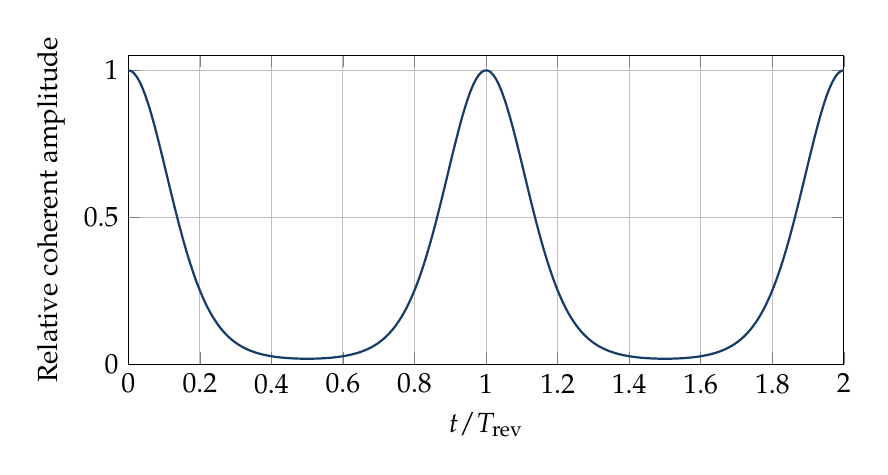
\begin{tikzpicture}\begin{axis}[width=.88\linewidth,height=5.5cm,xlabel={$t/T_{\rm rev}$},ylabel={Relative coherent amplitude},xmin=0,xmax=2,ymin=0,ymax=1.05,grid=major]
\addplot[deep,thick,domain=0:2,samples=250]{exp(2*(cos(deg(2*pi*x))-1))};
\end{axis}\end{tikzpicture}\end{center}
The collapse--revival phenomenon was observed in ultracold atomic optical lattices by Greiner and colleagues in 2002. It is a direct manifestation of the quantized on-site interaction energy.
\section{How these quantities are measured}
\begin{itemize}
\item \textbf{Time-of-flight interference:} after releasing the lattice, diffraction-peak contrast probes spatial coherence $\langle a_i^\dagger a_j\rangle$; finite imaging resolution and envelope functions matter.
\item \textbf{Number-resolved microscopy:} appropriate lattice microscopes can infer site occupations and number correlations, subject to parity and detection restrictions of particular implementations.
\item \textbf{Modulation spectroscopy:} periodic modulation of $J$ or $U$ can excite gapped particle--hole modes and reveal spectral response.
\item \textbf{Quench dynamics:} changing lattice depth on controlled timescales measures oscillations, correlation growth, collapse and revival.
\end{itemize}
\section{Model limits and interpretation}
The Bose--Hubbard parameters are derived under a single-band, localized-Wannier approximation. Higher bands, trapping inhomogeneity, density-dependent tunneling, finite temperature, loss and long-range interactions can change the quantitative predictions. The coherence discussed throughout is the center-of-mass lattice coherence of composite bosonic atoms, \emph{not} the electronic overlap producing bands in a conventional solid.
\section{Additional exercises}
\begin{enumerate}
\item Derive the $3\times3$ dimer Hamiltonian directly from the ladder operators.
\item Derive normalized dimer eigenvectors for arbitrary $U/J$ and verify orthogonality.
\item Prove the one-body natural occupations $1\pm4J/D$.
\item Compute the entanglement entropy between the two wells for the dimer ground state.
\item Enumerate the $N=3,L=3$ basis and all nonzero hopping matrix elements.
\item Obtain the particle--hole dispersions to first order in $J/U$.
\item Derive the small-wavevector lattice phonon velocity.
\item Derive the single-site mean-field critical line and its lobe tip.
\item Starting with the quench initial state, compute the two-site oscillation $P_{11}(t)$.
\item Derive collapse--revival periodicity for a coherent onsite state and discuss number-squeezed initial states.
\end{enumerate}
\section*{Selected references}
\begin{enumerate}
\item Greiner, M., Mandel, O., Esslinger, T., H\"ansch, T. W., Bloch, I. ``Quantum phase transition from a superfluid to a Mott insulator in a gas of ultracold atoms.'' \emph{Nature} \textbf{415}, 39--44 (2002). DOI: \href{https://doi.org/10.1038/415039a}{10.1038/415039a}.
\item Greiner, M., Mandel, O., H\"ansch, T. W., Bloch, I. ``Collapse and revival of the matter wave field of a Bose--Einstein condensate.'' \emph{Nature} \textbf{419}, 51--54 (2002). DOI: \href{https://doi.org/10.1038/nature00968}{10.1038/nature00968}.
\item Capogrosso-Sansone, B., Prokof'ev, N. V., Svistunov, B. V. ``Phase diagram and thermodynamics of the three-dimensional Bose--Hubbard model.'' \emph{Phys. Rev. B} \textbf{75}, 134302 (2007). DOI: \href{https://doi.org/10.1103/PhysRevB.75.134302}{10.1103/PhysRevB.75.134302}.
\item Fisher, M. P. A. et al., ``Boson localization and the superfluid-insulator transition.'' \emph{Phys. Rev. B} \textbf{40}, 546--570 (1989).
\end{enumerate}

\clearpage
\section*{Supplementary Sections to Chapter IV: deeper explanations (original chapter preserved)}
\addcontentsline{toc}{section}{Supplementary Sections to Chapter IV}
\subsection*{IV-A. The exact eigenvectors, not just eigenvalues}
For two bosons in two sites, introduce $|S\rangle=(|20\rangle+|02\rangle)/\sqrt2$, $|A\rangle=(|20\rangle-|02\rangle)/\sqrt2$. In the $\{|S\rangle,|11\rangle\}$ block the Hamiltonian is $\begin{psmallmatrix}U&-2J\\-2J&0\end{psmallmatrix}$. With $D=\sqrt{U^2+16J^2}$, the normalized repulsive-ground-state vector is $|G\rangle=\sqrt{(1-U/D)/2}|S\rangle+\sqrt{(1+U/D)/2}|11\rangle$. This expression makes all occupation probabilities, coherences, number fluctuations and site entanglement calculable in closed form.
\begin{supplexample}[Ground-state probabilities at $U/J=4$]
We have $D=4\sqrt2 J$, so $P_{11}=(1+1/\sqrt2)/2\simeq0.85355$. Each double-occupied configuration has probability $(1-P_{11})/2\simeq0.07322$. These probabilities sum to unity and give the entire diagonal occupation distribution.
\end{supplexample}
\subsection*{IV-B. Finite-size crossover versus thermodynamic transition}
For any generic finite system with a nondegenerate ground state separated from excited states, observables vary smoothly with parameters. A nonanalytic zero-temperature quantum critical point emerges only after taking a suitable thermodynamic limit. The two-site change from a bonding state to $|11\rangle$ is a crossover, not a genuine phase transition. In a large lattice with integer filling, the transition can be located using gaps, compressibility, long-distance correlations, finite-size scaling, or quantum Monte Carlo.
\subsection*{IV-C. Particle--hole excitation and the atomic limit}
At unit filling with $J=0$, moving an atom from one site to another turns $|1,1\rangle$ into $|0,2\rangle$ and costs exactly $U$. For nonzero $J$, particle and hole branches acquire dispersion and the neutral gap is modified. It is generally incorrect to identify the many-body excitation gap with $U$ for every $J/U$ or near the transition. The chemical-potential particle/hole gaps and fixed-particle-number neutral gap are related but not identical notions.
\subsection*{IV-D. Mean-field predictions versus low-dimensional physics}
Site-factorized mean field is useful for a qualitative phase diagram but becomes less accurate in one dimension or near criticality. In one dimension the integer-filling superfluid--Mott transition has Berezinskii--Kosterlitz--Thouless character, whereas higher-dimensional cases have different universality behavior at the lobe tip. The numerical critical ratio depends on lattice dimension, coordination, filling, trapping inhomogeneity and Hamiltonian conventions.
\subsection*{IV-E. Corrections for quench interpretation}
For a sudden $U_i=0\to U_f$ quench with unchanged $J$ in the exactly two-site/two-atom model, the initial state is $|G_i\rangle=(|S\rangle+|11\rangle)/\sqrt2$. With $D_f=\sqrt{U_f^2+16J^2}$ one obtains
\begin{equation}
P_{11}(t)=\frac12+\frac{2JU_f}{D_f^2}\left[1-\cos(D_f t/\hbar)\right].
\end{equation}
The formula depends on this particular initial state and assumes an isolated sudden quench; it should not be confused with the deep-lattice collapse--revival formula derived from an onsite coherent state at $J\simeq0$.
\subsection*{IV-F. Two independent observables}
For the same ground state, $C=\langle a_L^\dagger a_R\rangle=4J/D$ and $\langle(n_L-n_R)^2\rangle=2(1-U/D)$. Both fall as repulsive $U/J$ increases. The relationship is not universal across all states: a quenched or thermally mixed state can exhibit different coherence and fluctuation dynamics. Chapter V develops reduced density matrices to distinguish correlations from entanglement.

\end{document}
